\documentclass[10pt,a4paper]{article}
\usepackage[utf8]{inputenc}
\usepackage{amsmath}
\usepackage{amsfonts}
\usepackage{amssymb}
\usepackage{graphicx}
\usepackage{pdfpages}



\author{Helena Brekalo and Annelies Faes}


\begin{document}

\begin{titlepage}

\newcommand{\HRule}{\rule{\linewidth}{0.5mm}} % Defines a new command for the horizontal lines, change thickness here

\center % Center everything on the page
 
\textsc{\LARGE KU Leuven}\\[1.5cm] % Name of your university/college


\begin{figure}[ht!]
\centering

\includegraphics[width=30mm]{logo_theo.png}
\label{kulogo}
\end{figure}

\textsc{\Large Distributed Systems}\\[0.5cm] % Major heading such as course name


\HRule \\[0.4cm]
{ \huge \bfseries Java RMI report}\\[0.4cm]
\HRule \\[1.5cm]


\textsc{\large Ma Ingenieurswetenschappen: Computerwetenschappen}\\[0.5cm] % Minor heading such as course title


\Large \emph{Author:}\\
Helena \textsc{Brekalo}\\
Annelies \textsc{Faes}\\[2cm]


{\large 2015-2016}\\[3cm] % Date

\vfill % Fill the rest of the page with whitespace

\end{titlepage}
\clearpage

\section{Overview}
The application consists of three parts: the rental part where the companies are located, the agency and the client. 
As stated in the assignment, each company can run on its own server. Located on these servers are all classes related to the company. The second part consists of the agency, all session-related classes and the RMI registry. The third part consists of the client.\\
The RMI registry manages the stubs of the companies and the session manager. To use the application, a session has to be requested. The client requests either a reservation session or a manager session from the session manager through the stub of the session manager, which it acquired through the RMI registry. The session manager returns a stub of the requested session. All communication happens through these sessions via their stubs. 


\section{Design decisions}
\subsection{Remotely accessible classes}


\paragraph{Host: rental}
\begin{itemize}
\item \textbf{CarRentalCompany:} This class is remotely accessible through the ICarRentalCompany interface. It is the central point on the rental host of the company and contains most of the logic of that company that classes on other hosts need to be able to use. Multiple sessions need to be able to access the company simultaneously. They need to have information about the state in which other clients left the company (e.g. rented a car).
\end{itemize}

\paragraph{Host: agency}
\begin{itemize}
\item \textbf{SessionManager:} This class is remotely accessible through the ISessionManager interface. The session manager needs to be remotely accessible for all clients that want to use the application. The session manager will provide the clients with a session (a manager session or a reservation session) through which they get the functionality they need.
\item \textbf{ManagerSession:} This class is remotely accessible through the IManagerSession interface. Through this class, managers get the functionality they need to manage their company. The manager session needs to be accessible by any client.
\item \textbf{ReservationSession:} This class is remotely accessible through the IReservationSession interface. Through this class, renters get the functionality they need to rent a car. The reservation session needs to be accessible by any client.
\end{itemize}

The CarRentalCompany objects are located on the company server. They can all be located at a different server as stated in the assignment.\\
The agency is located on another host because it is a central point where all companies can be managed and  it is able to control which functionality is accessible by clients by means of sessions.\\

The CarRentalCompany and SessionManager objects are registered via the built-in RMI registry. The sessions themselves are not registered via the built-in RMI registry for life cycle management purposes. See subsection \ref{lifecycle}.

\subsection{Serializable classes}
%TODO which classes are serializable and why?

\paragraph{Host: rental}
\begin{itemize}
\item \textbf{Quote:} Quotes are created by the CarRentalCompany and all quotes from the same client are kept in the ReservationSession of that client. Because of that, the quote objects need to be sent over the wire.
\item \textbf{Reservation:} Reservations are created at the company and are sent back over the wire to the client. 
\end{itemize}

\paragraph{Host: agency}
\begin{itemize}
\item \textbf{ReservationConstraints:} In order to create a quote (which is requested by the client), reservation constraints are needed, so the ReservationConstaints objects need to be sent from the agency to the client. %Waarom niet meer bij de client?
\end{itemize}

\subsection{Life cycle management of sessions}
\label{lifecycle}
Sessions are created by the session manager, their stub is returned to the client. The client keeps a reference as long as it's needed. When the client doesn't have a reference for the stub anymore, the garbage collector will automatically remove the unused sessions.

\subsection{Synchronization}

%TODO At which places is synchronization necessary to achieve thread-safety? Will those places become a bottleneck by applying synchronization?

\paragraph{Host: agency}
\begin{itemize}
\item \textbf{Agency:} The methods getCheapestCarType and checkForAvailableCarTypes both contain a period in which the request needs to be checked. If at the time of checking confirmQuotes is executed, the results of the methods may be inconsistent with the actual values.\\ 
The methods getNbOfReservationsBy, getNbOfReservationsForCarType and getMostPopularCarRentalCompany could return a wrong amount of reservations or the wrong most popular car rental company because a writing operation might be going on at the same time. In the case of reservations, the wrong totals might be returned if cancellations happen in confirmQuotes at or after the time of reading.
\item \textbf{ReservationSession:} The method confirmQuotes needs to be synchronized because if one of the confirmations fails, a rollback is needed, so the reservations made up until that point need to be cancelled. No other method should be able to access the reservations before the confirmation is complete.
\end{itemize}

\section{Diagrams}

\subsection{Full class diagram}
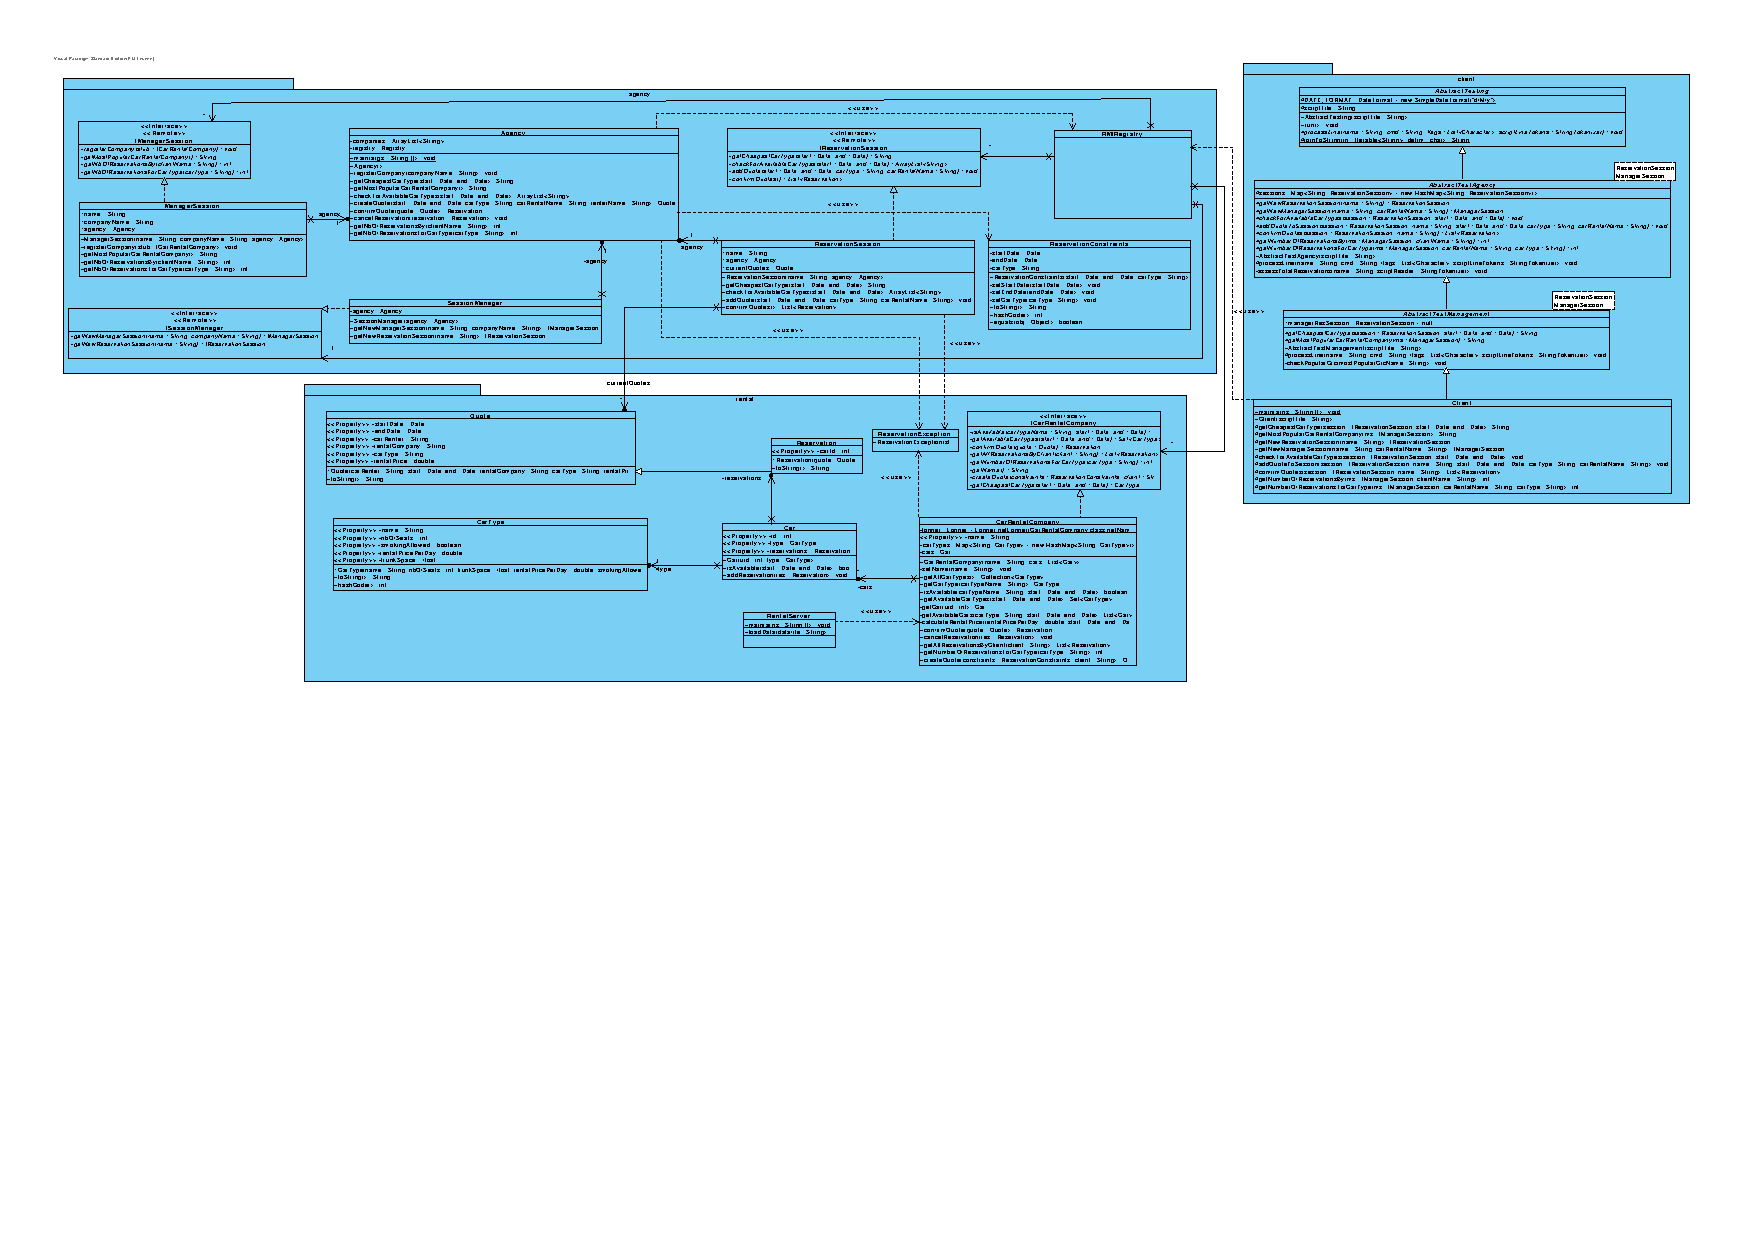
\includepdf[pages={1}, landscape]{CarRentalApplicationClassDiagram.pdf} 
\clearpage

\subsection{Deployment diagram}
\begin{figure}[ht!]
\centering
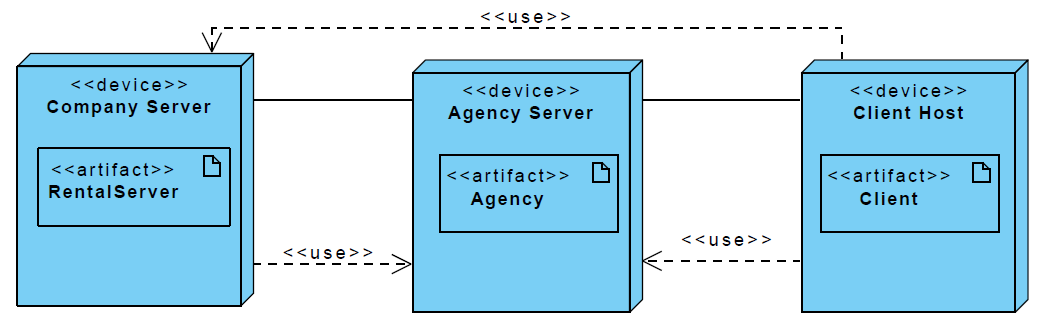
\includegraphics[width=160mm]{DeploymentDiagram.png}
\label{deploymentdiagram}
\end{figure}

\clearpage

\subsection{Sequence diagrams}

\begin{figure}[ht!]
\centering
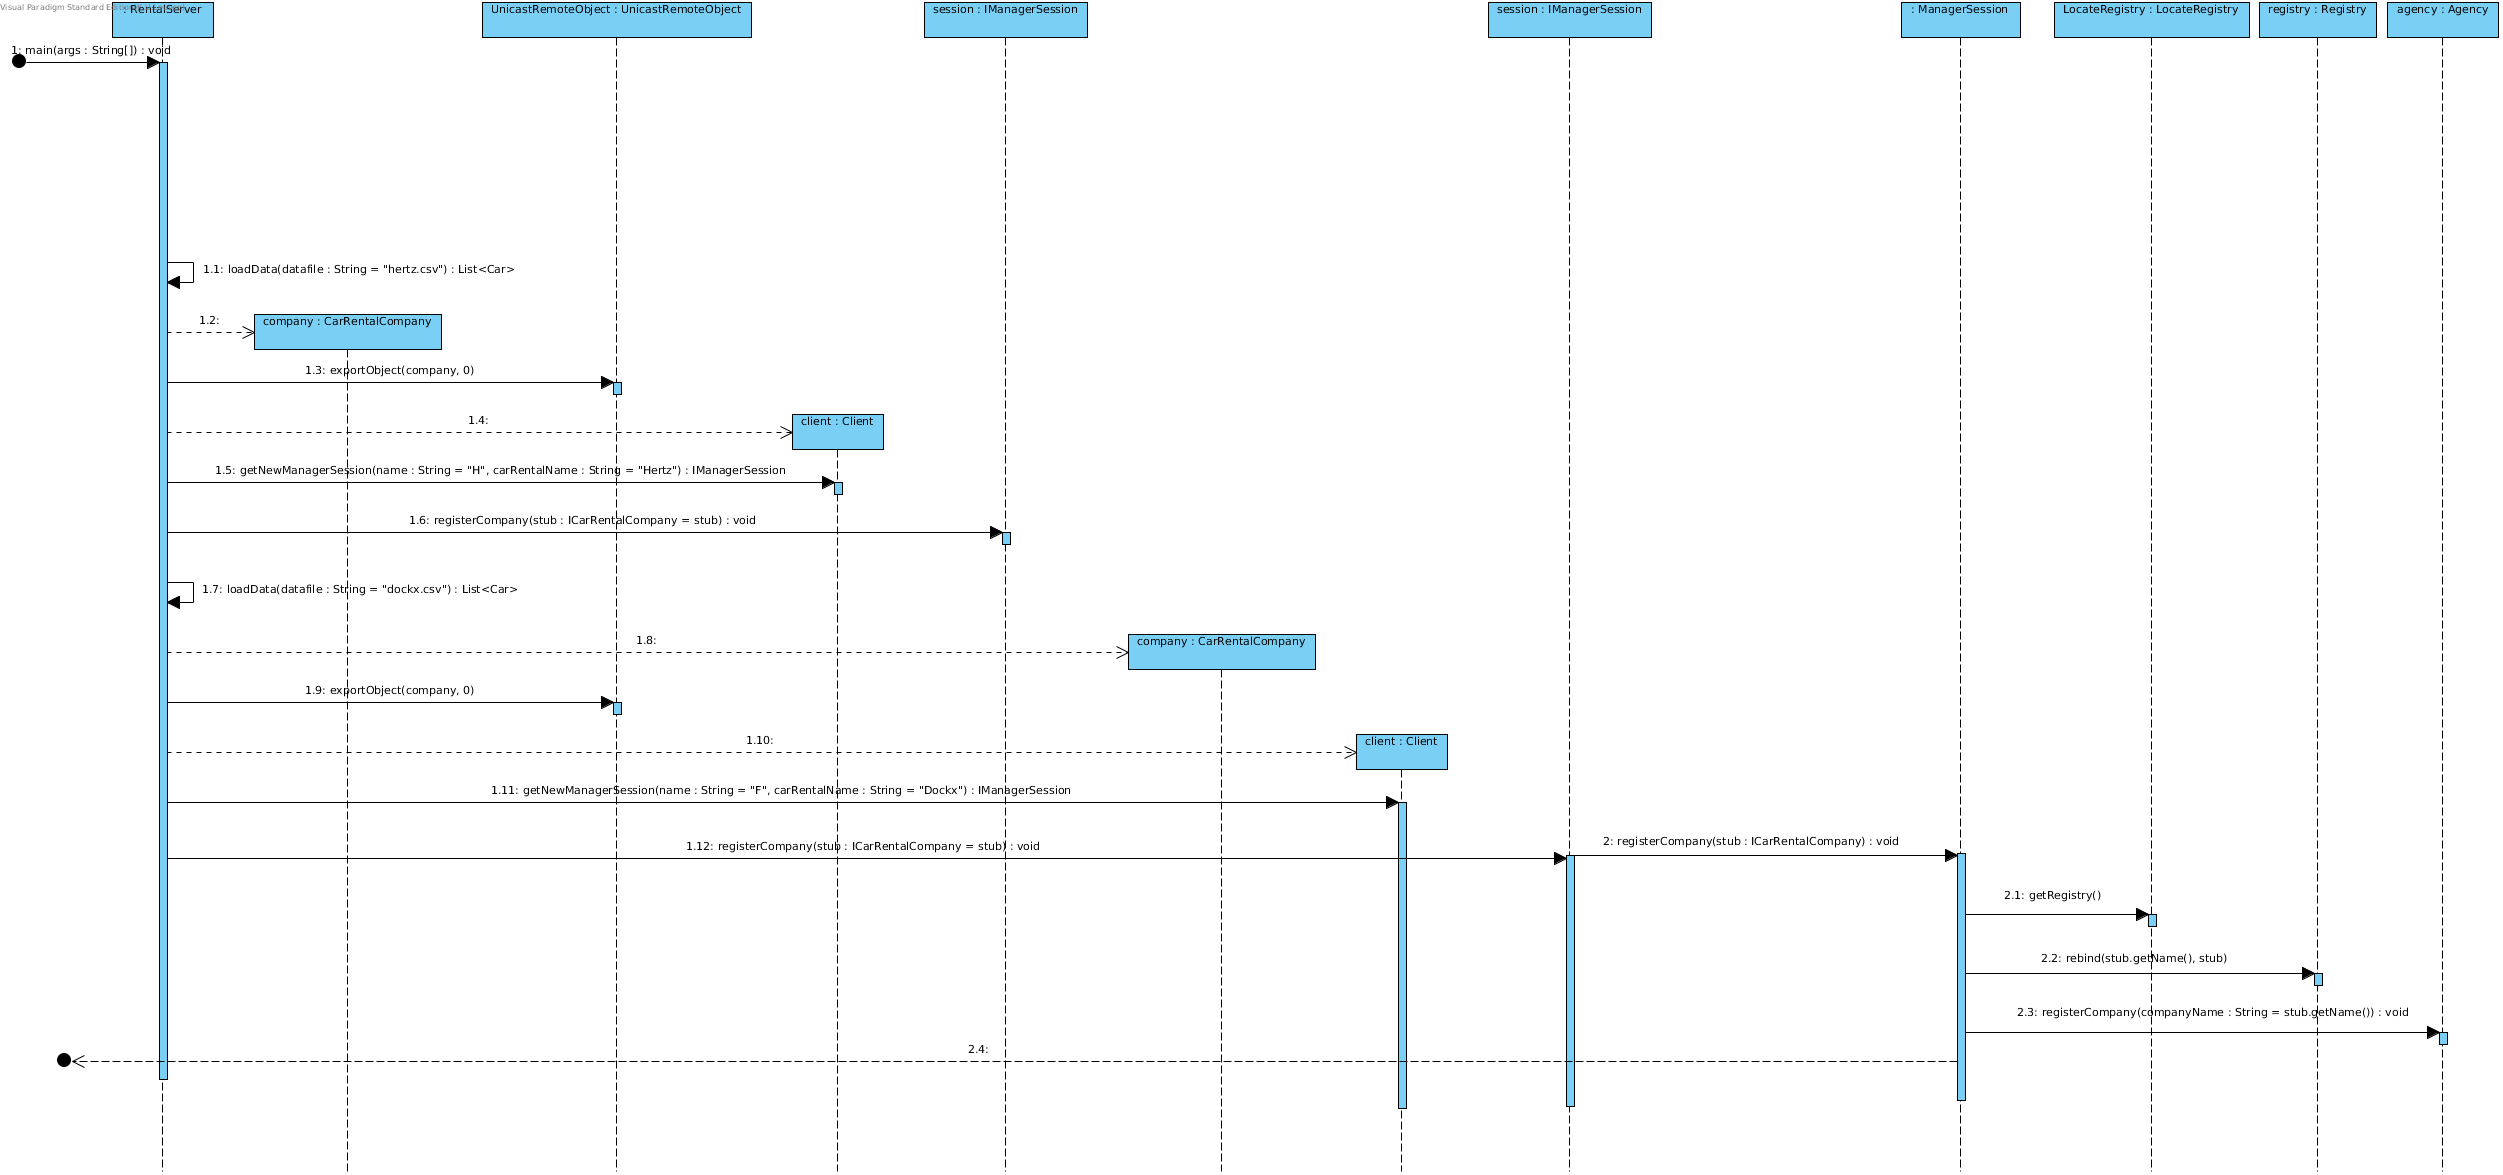
\includegraphics[width=160mm]{registerCompany.png}
\caption{Create and register a company.} 
\end{figure}

\begin{figure}[ht!]
\centering
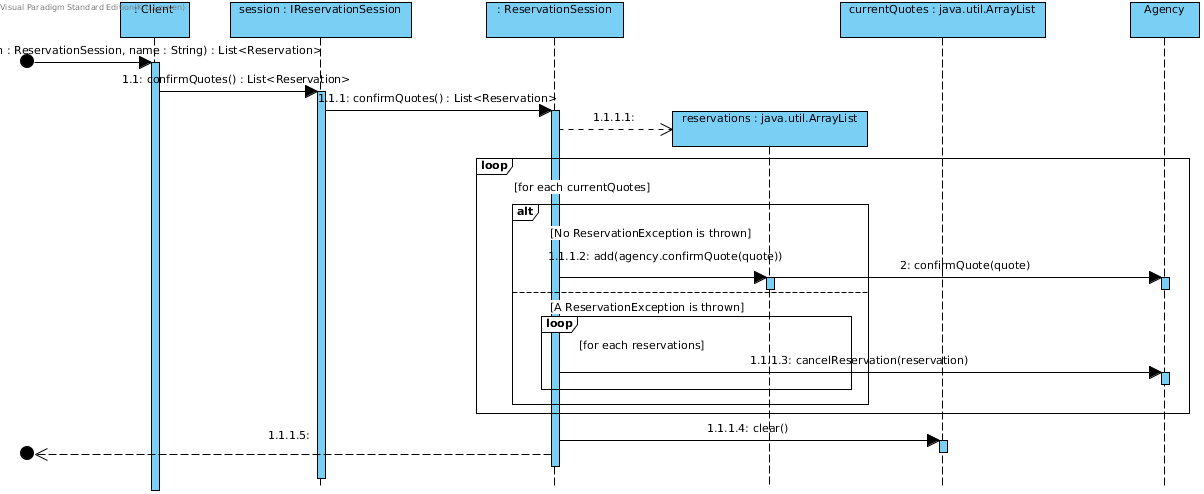
\includegraphics[width=160mm]{confirmQuotes.png}
\caption{Confirm all quotes in a session.} 
\end{figure}

\end{document}